\chapter{Previous Research} \label{prev-res}

The subject of using Trusted Execution Environments to protect IP of ML models has been researched a little in the past. This chapter partly answers to the \ref{rq1}.

There are at least three papers published specifically on the subject; \textit{SecureTF: A Secure TensorFlow Framework (2020)}\cite{securetf}, \textit{Using Intel SGX to Improve Private Neural Network Training and Inference (2020)}\cite{usingsgx} and \textit{Securely Exposing Machine Learning Models to Web Clients using Intel SGX (2019)\cite{securely}}. However, none of these papers discusses specifically the problem when the ML application is distributed entirely to the end-users.

This chapter also mentions two other studies which are related, but whose objectives did not include protection of machine learning models. Gramine Project\cite{gramine}, which includes two papers and framework software, is mentioned first and then paper \textit{SGXCrypter: IP protection for portable executables using Intel's SGX technology (2017)}\cite{sgxcrypter}. Although their goal is not specifically to protect machine learning models, they still can be considered relevant.

\subsubsection{SecureTF: A Secure TensorFlow Framework} \label{securetfa}

\textit{SecureTF: A Secure TensorFlow Framework} by Roland Kunkel, Franz Gregor and Do Le Quoc from TU Dresden, Sergei Arnautov and Christof Fetzer from Scontain UG and Pramod Bhatotia from University of Edinburgh provides a complete, ready-to-use framework to use a popular and open-source machine learning and artificial intelligence library TensorFlow securely with Trusted Execution Environments. Because the machine learning operations require a lot of computation power, the machine learning operations are often done on third-party cloud infrastructure.

The main concern of the writers of this paper was how to do machine learning operations securely in the untrusted cloud environment. The paper investigates the training phase as well as the classification phase of the machine learning process. In the training phase, the datasets used to train the model can be considered information that must be protected. On the other hand, in the classification phase, the model itself becomes valuable intellectual property and can be considered information that must be protected.

As a solution to this concern, the writers of this paper propose SecureTF, a framework which bundles the machine learning application with all needed libraries into a software that is transferred to the TEE enclave in its entirety. Machine learning models and training data provided to the enclave encrypted, which are then decrypted inside the enclave after successful remote attestation. The high-level system overview can be seen in Figure \ref{img:securetf}.

\begin{figure}
\centering 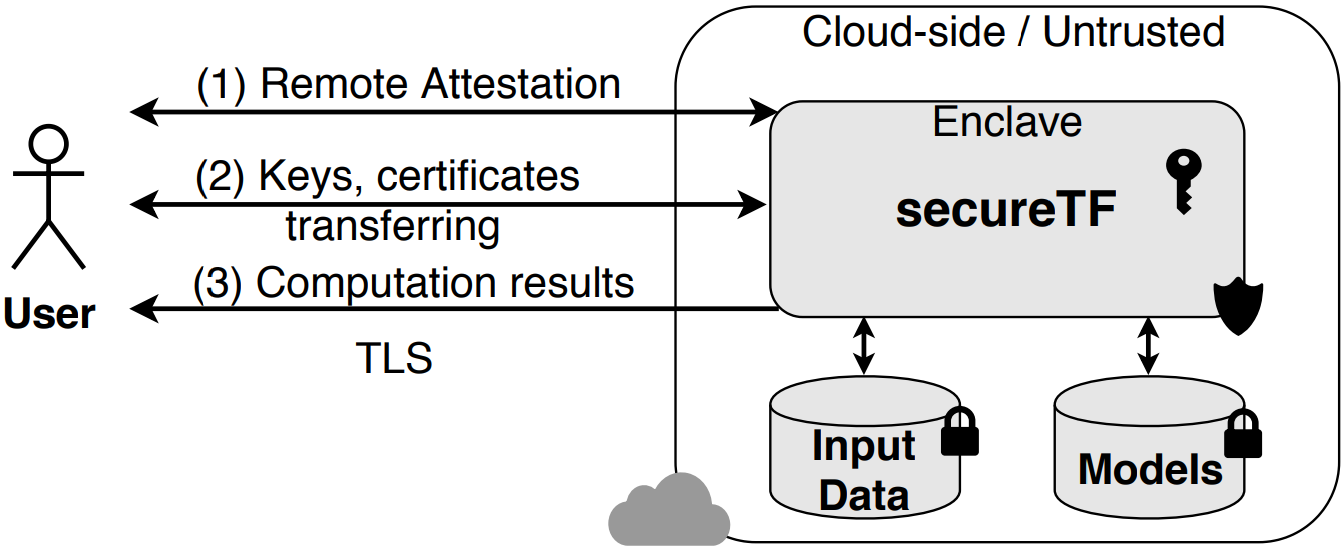
\includegraphics[width=0.7\textwidth]{img/securetf}
\caption{System overview of SecureTF from \textit{SecureTF: A Secure TensorFlow Framework}}
\label{img:securetf} 
\end{figure}

The same authors also earlier wrote \textit{TensorSCONE: A Secure TensorFlow Framework using Intel SGX}\cite{tensorscone} that is focused on the same concerns, but the implementation was specifically done for Intel SGX.

\subsubsection{Using Intel SGX to Improve Private Neural Network Training and Inference} \label{improveprivate}

\textit{Using Intel SGX to Improve Private Neural Network Training and Inference} by Ryan Karl, Jonathan Takeshita and Taeho Jung from University of Notre Dame is a bit shorter paper where the main focus is on the running the inference phase of the Deep Neural Network (DNN) machine learning algorithm in an untrusted cloud infrastructure.

The approach is more theoretical and proposes a mathematical method which includes encrypting to run machine learning inference securely in an untrusted environment. There is no implementation discussed.

\subsubsection{Securely Exposing Machine Learning Models to Web Clients using Intel SGX} \label{securelyexposingml}
 
\textit{Securely Exposing Machine Learning Models to Web Clients using Intel SGX} by Dávid Ács and Adrian Coleşa from Technical University of Cluj-Napoca discusses the possibility to serve the machine learning model as a part of a web application, but still keeping it secure. Their main concern is that even though the server infrastructure could be considered secure, there might be latency and performance loss when the machine learning application is used through the internet, in a web application.

The method proposed in this paper is to serve the machine learning application and related models to the client's web browser. The web browser initializes an Intel SGX enclave, where the confidential data can be processed securely, without exposing them outside the enclave. The proposed method includes a web page, browser extension, native client-side application, server and usage of Intel's Remote Attestation. The client must fully support Intel SGX. The architecture overview can be seen in Figure \ref{img:websgx}.

\begin{figure}
\centering 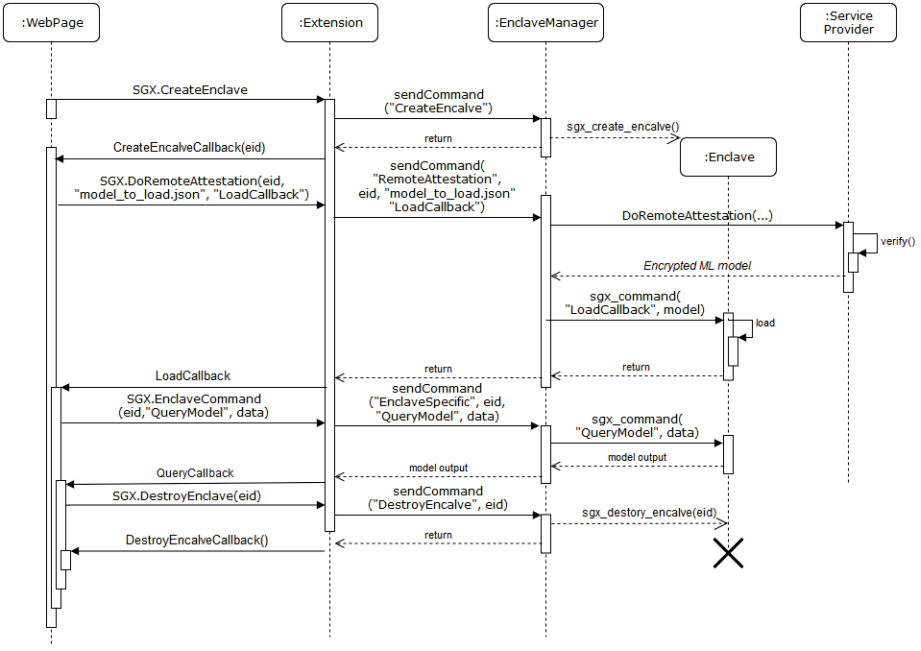
\includegraphics[width=0.8\textwidth]{img/websgx}
\caption{Query and load sequence diagram of proposed method from \textit{Securely Exposing Machine Learning Models to Web Clients using Intel SGX}}
\label{img:websgx} 
\end{figure}

\subsubsection{Gramine Project} \label{prevgramine}

Gramine Project, originally launched by OSCAR LAB at Stony Brook University, has become an important part of this thesis. Gramine, which was originally called Graphene, is a library operating system (LibOS) with Intel SGX support which is perfectly suitable for protecting intellectual property of ML models. Gramine will be discussed in detail in Section \ref{gramine}.

Gramine team has published two papers regarding their project; \textit{Cooperation and Security Isolation of Library OSes for Multi-Process Applications (2014)}\cite{graminepaper} and \textit{Graphene-SGX: A Practical Library {OS} for Unmodified Applications on SGX (2017)}\cite{graminesgxwp}.

\begin{figure}
\centering 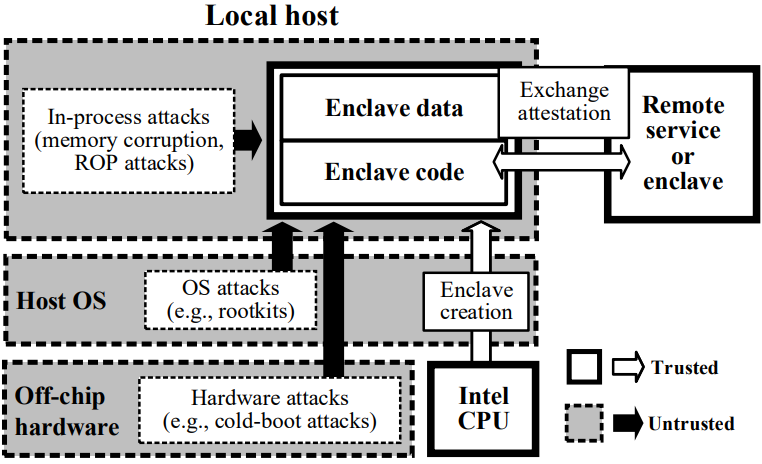
\includegraphics[width=0.7\textwidth]{img/graminethreat}
\caption{The threat model of SGX, presented in \textit{Graphene-SGX: A Practical Library {OS} for Unmodified Applications on SGX}. Intel SGX protects applications from three types of attacks: in-process attacks from outside the enclave, attacks from the OS or hypervisor, and attacks from off-chip hardware.}
\label{img:threatmodel} 
\end{figure}

\subsubsection{SGXCrypter: IP protection for portable executables using Intel's SGX technology} \label{sgxcrypter}

One research that can be considered relevant from the perspective of protecting machine learning models is \textit{SGXCrypter: IP protection for portable executables using Intel's SGX technology} by Dimitrios Tychalas and Michail Maniatakos from New York University Abu Dhabi and Nektarios Georgios Tsoutsos from NYU Tandon School of Engineering. The main concern of this study was the compromised intellectual property through reverse engineering. The existing techniques to make reverse engineering impossible, such as data obfuscation, have been found unsuitable, especially because data obfuscation is a common technique used by malware authors. Antivirus engines often consider executables with obfuscated data as a malicious software.

The paper proposes a special encryption schema to encrypt Microsoft Windows software executables. Windows software executables have an encrypted payload section that can be decrypted by the client's Trusted Execution Environment -- Intel SGX enclave. By using this approach, anything inside the executables encrypted payload, for example a machine learning model, is never exposed to the other parts of the client's system.